
\section{Results}
\label{sec:results}

The data and SM prediction are shown in Fig.~\ref{fig:pfmet_eemm}, and split between the $ee$ (Fig.~\ref{fig:pfmet_ee})
and $\mu\mu$ (Fig.~\ref{fig:pfmet_mm}) final states. We observe 7  events (all in the $\mu\mu$ channel) in the loose signal 
region (MET $>$ 60 GeV), compared to a data-driven prediction of $6.0 \pm 0.8$, which is dominated by the estimated 
\ttbar contribution. For the tight signal region defined by MET $>$ 120 GeV, we observe 0 events compared to a 
data-driven prediction of $1.2 \pm 0.4$. These uncertainties are statistical only, systematic uncertainties will be 
discussed in Sec.~\ref{sec:systematics}. We conclude that no excess of signal with respect to the data-driven prediciton is observed.

When we have enough data, we will display in the figures the predicted $t\bar{t}$ MET distribution obtained by scaling the $e\mu$ distribution
in data. However, due to limited statistics we cannot currently do this. Therefore for display purposes only, we have taken the
$t\bar{t}$ MET distribution from MC and normalized it such that the integral for MET$>60$~GeV matches the data-driven prediction
from the OF subtraction. 
%{\bf I don't know if we want to do this in the final plots.}

%We observe a slight excess of observed
%MET with respect to the data driven prediction in the bulk of the distribution. Systematic effects which may contribute
%to this excess, including lepton mismeasurement and effects related to pile up, will be assessed in Sec.~\ref{sec:systematics}.

%note on my (Warren's) plot naming convention:
% the plots which have 'all' in the title are NOT binned in vsjp.
% ie 'pfMET_pred_2ge_alleb_log.png'
% I will leave the ones which are binned in vsjp in cvs, but remove from note (ie pfMET_pred_2_eb_log.png)

\begin{figure}[hbtp]
  \begin{center}
    \resizebox{1.0\linewidth}{!}{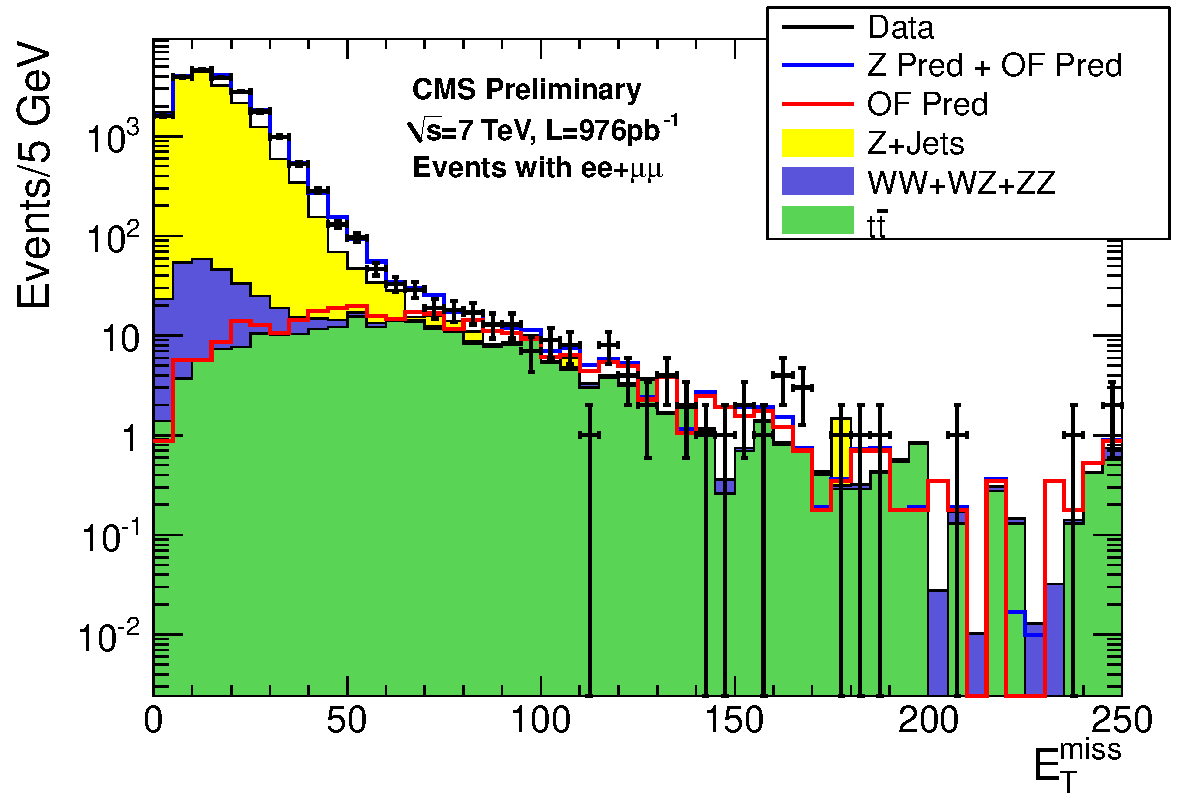
\includegraphics{plots/lep_metPredicted.pdf}}
	\\ \medskip 
    %\resizebox{\linewidth}{!}{
    \begin{tabular}{lccc}
\hline
                        &   N(MET $>30$)  GeV    &   N(MET $>60$)  GeV    &   N(MET $>120$) GeV   \\
\hline
              Z pred    &  38.47  $\pm$  0.90    &   1.81  $\pm$  0.13    &   0.14  $\pm$  0.03   \\
                OFOS    &   6.43  $\pm$  1.00    &   4.24  $\pm$  0.82    &   1.10  $\pm$  0.42   \\
\hline
       Z pred + OFOS    &  44.90  $\pm$  1.35    &   6.04  $\pm$  0.82    &   1.24  $\pm$  0.42   \\
\hline
                data    &                  51    &                   7    &                   0   \\
\hline
    \end{tabular}
    \caption{
      The observed MET distribution for data in the $ee$ and $\mu\mu$ channels (black points),
      predicted $t\bar{t}$ MET distribution (red line), the sum of predicted $t\bar{t}$ MET distribution and
      Z  MET  distribution  predicted  from photon  MET  templates
      (solid blue line),  and MC stacked. Here $VV$  indicates the sum
      of  $WW$,  $WZ$  and  $ZZ$, while  additional  backgrounds  from
      $W+$jets   and   single  top   are   omitted   since  they   are
      negligible.  Below the  plot is  tabulated the  integral  of the
      predicted  MET distribution  using the  MET templates  method (Z
      pred),  the  predicted ttbar  yield  using  the opposite  flavor
      subtraction  technique (OFOS), the  sum of  these two
      contributions (Z pred + OFOS), and the observed MET distribution
      (data), for  MET $>$ 30~GeV,  $>$ 60~GeV and $>$  120~GeV. The
      quantity pull  = (data-Z prediction)/(Z prediction)  is shown on
      top  of the  plot.  
    }
    \label{fig:pfmet_eemm}
  \end{center}
\end{figure}

\begin{figure}[hbtp]
  \begin{center}
    \resizebox{1.0\linewidth}{!}{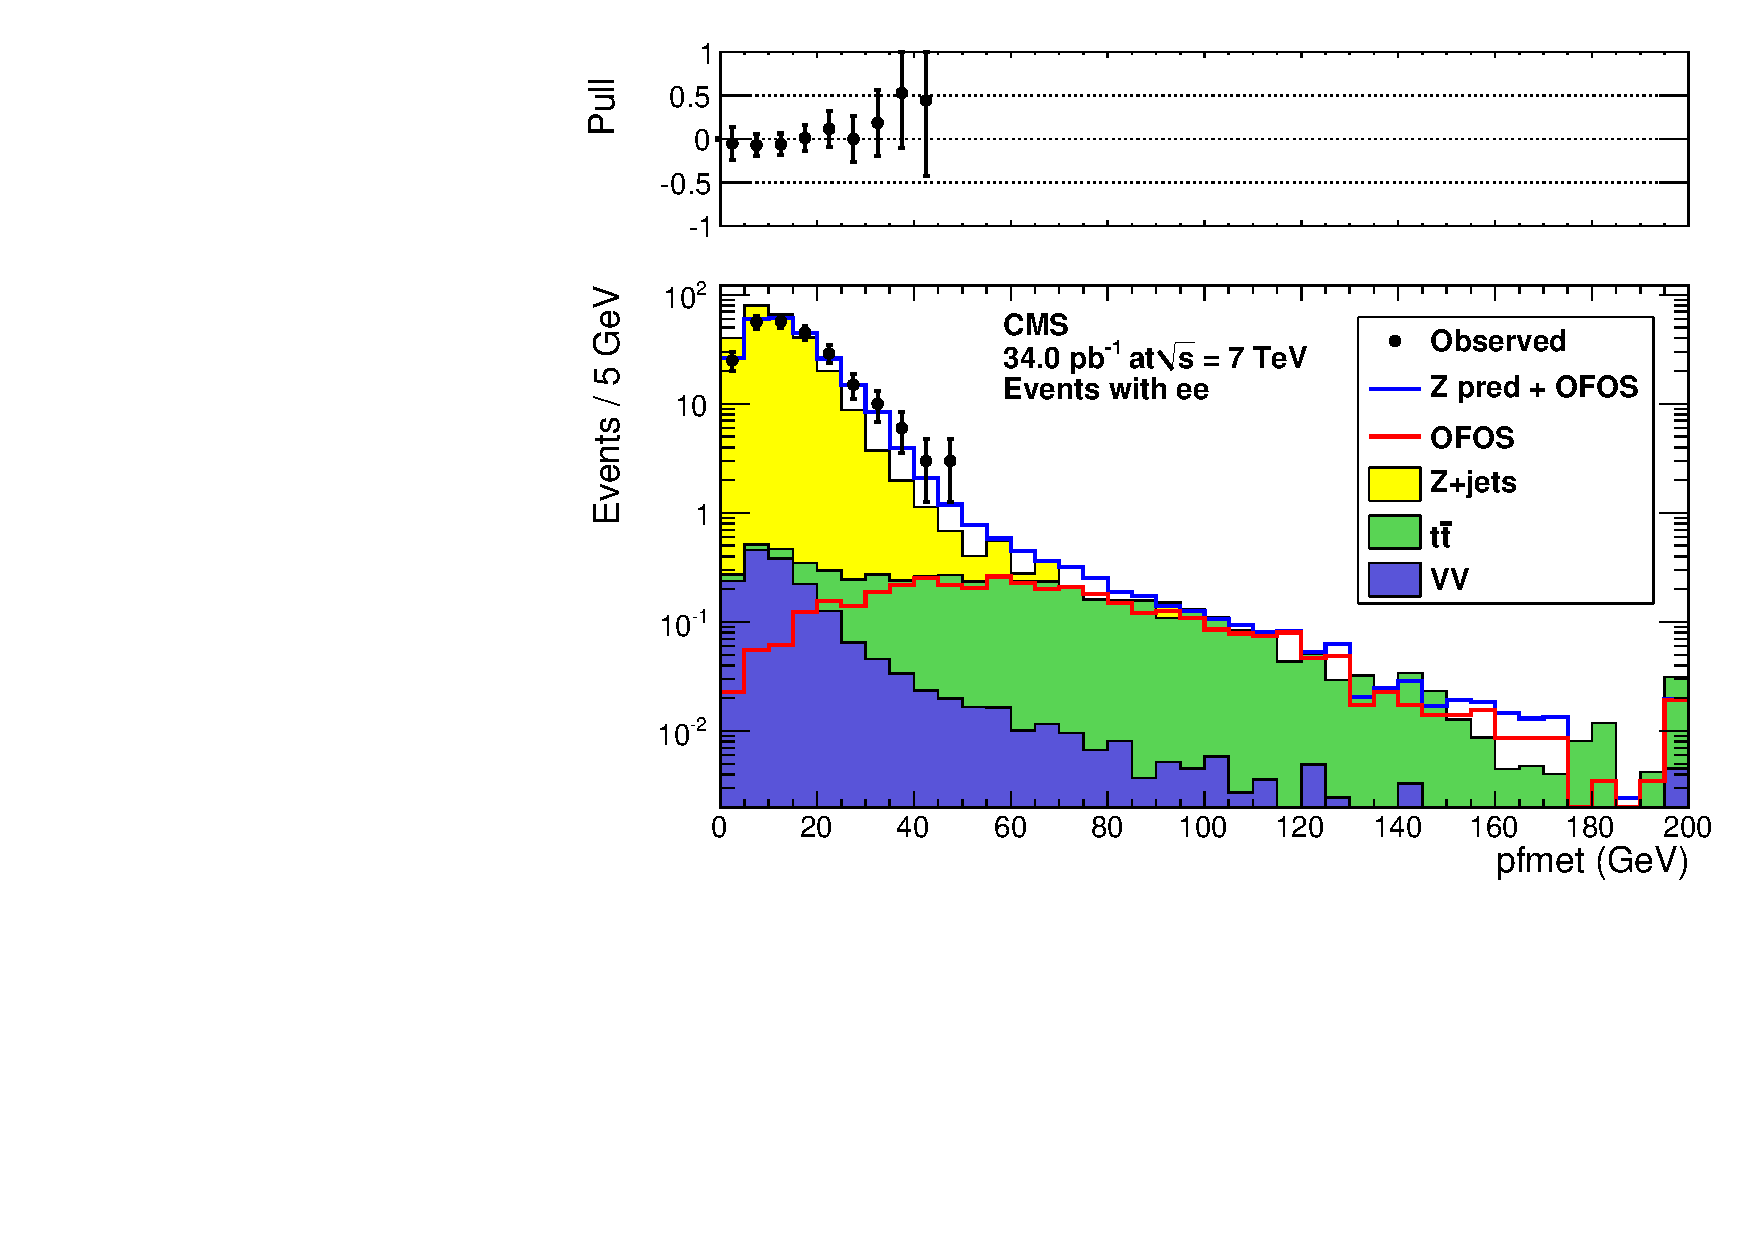
\includegraphics{plots/lep_metPredicted_ee.pdf}}
	\\ \medskip 
    %\resizebox{\linewidth}{!}{
    \begin{tabular}{lccc}
\hline
                        &   N(MET $>30$)  GeV    &   N(MET $>60$)  GeV    &   N(MET $>120$) GeV   \\
\hline
              Z pred    &  16.45  $\pm$  0.37    &   0.79  $\pm$  0.05    &   0.06  $\pm$  0.01   \\
                OFOS    &   2.88  $\pm$  0.45    &   1.90  $\pm$  0.36    &   0.49  $\pm$  0.19   \\
\hline
       Z pred + OFOS    &  19.32  $\pm$  0.58    &   2.68  $\pm$  0.37    &   0.56  $\pm$  0.19   \\
\hline
                data    &                  22    &                   0    &                   0   \\
\hline
    \end{tabular}
    \caption{
      The observed MET distribution for data in the $ee$ channel (black points),
      predicted $t\bar{t}$ MET distribution (red line), the sum of predicted $t\bar{t}$ MET distribution and
      Z  MET  distribution  predicted  from photon  MET  templates
      (solid blue line),  and MC stacked. Here $VV$  indicates the sum
      of  $WW$,  $WZ$  and  $ZZ$, while  additional  backgrounds  from
      $W+$jets   and   single  top   are   omitted   since  they   are
      negligible.  Below the  plot is  tabulated the  integral  of the
      predicted  MET distribution  using the  MET templates  method (Z
      pred),  the  predicted ttbar  yield  using  the opposite  flavor
      subtraction  technique (OFOS), the  sum of  these two
      contributions (Z pred + OFOS), and the observed MET distribution
      (data), for  MET $>$ 30~GeV,  $>$ 60~GeV and $>$  120~GeV. The
      quantity pull  = (data-Z prediction)/(Z prediction)  is shown on
      top  of the  plot.  
    }
    \label{fig:pfmet_ee}
  \end{center}
\end{figure}

\begin{figure}[hbtp]
  \begin{center}
    \resizebox{1.0\linewidth}{!}{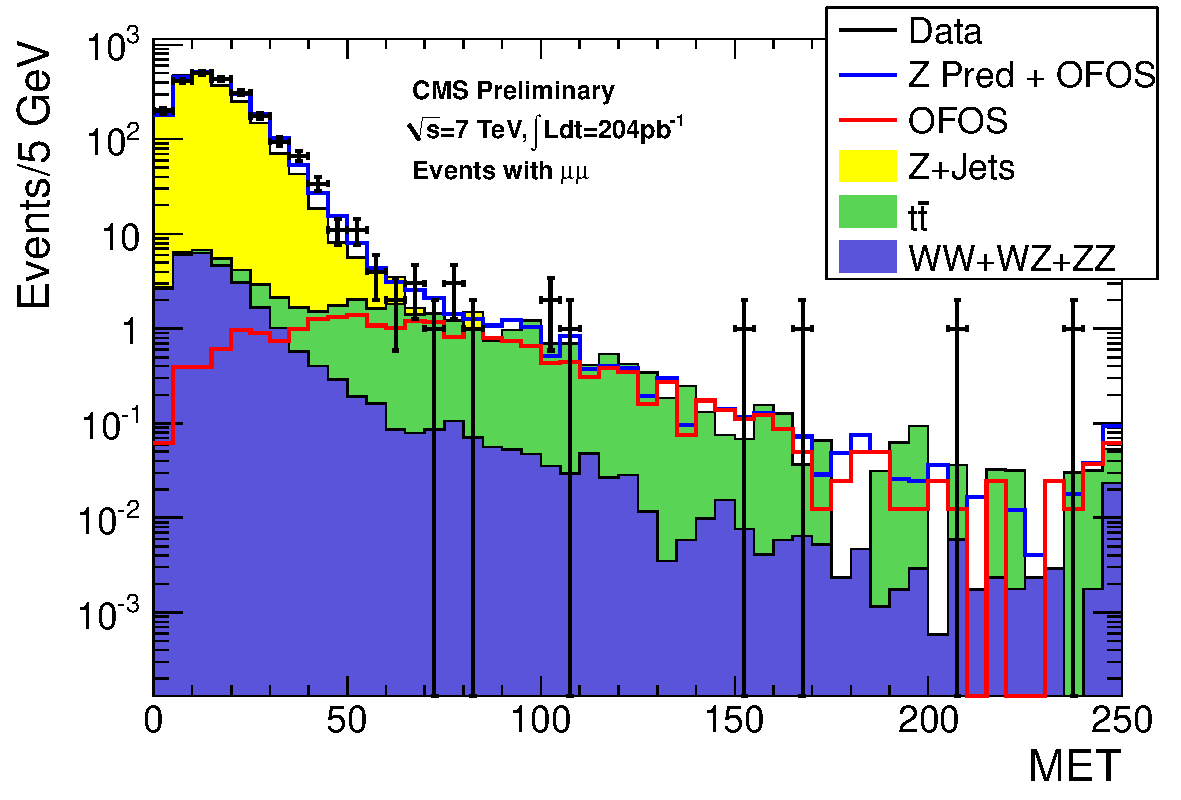
\includegraphics{plots/lep_metPredicted_mm.pdf}}
	\\ \medskip 
    %\resizebox{\linewidth}{!}{
    \begin{tabular}{lccc}
\hline
                        &   N(MET $>30$)  GeV    &   N(MET $>60$)  GeV    &   N(MET $>120$) GeV   \\
\hline
              Z pred    &  22.03  $\pm$  0.54    &   1.02  $\pm$  0.08    &   0.08  $\pm$  0.02   \\
                OFOS    &   3.55  $\pm$  0.55    &   2.34  $\pm$  0.45    &   0.61  $\pm$  0.23   \\
\hline
       Z pred + OFOS    &  25.58  $\pm$  0.77    &   3.36  $\pm$  0.46    &   0.68  $\pm$  0.23   \\
\hline
                data    &                  29    &                   7    &                   0   \\
\hline
    \end{tabular}
    \caption{
      The observed MET distribution for data in the $\mu\mu$ channel (black points),
      predicted $t\bar{t}$ MET distribution (red line), the sum of predicted $t\bar{t}$ MET distribution and
      Z  MET  distribution  predicted  from photon  MET  templates
      (solid blue line),  and MC stacked. Here $VV$  indicates the sum
      of  $WW$,  $WZ$  and  $ZZ$, while  additional  backgrounds  from
      $W+$jets   and   single  top   are   omitted   since  they   are
      negligible.  Below the  plot is  tabulated the  integral  of the
      predicted  MET distribution  using the  MET templates  method (Z
      pred),  the  predicted ttbar  yield  using  the opposite  flavor
      subtraction  technique (OFOS), the  sum of  these two
      contributions (Z pred + OFOS), and the observed MET distribution
      (data), for  MET $>$ 30~GeV,  $>$ 60~GeV and $>$  120~GeV. The
      quantity pull  = (data-Z prediction)/(Z prediction)  is shown on
      top  of the  plot.  
    }
    \label{fig:pfmet_mm}
  \end{center}
\end{figure}


